% Template for Cogsci submission with R Markdown

% Stuff changed from original Markdown PLOS Template
\documentclass[10pt, letterpaper]{article}

\usepackage{cogsci}
\usepackage{pslatex}
\usepackage{float}
\usepackage{caption}

% amsmath package, useful for mathematical formulas
\usepackage{amsmath}

% amssymb package, useful for mathematical symbols
\usepackage{amssymb}

% hyperref package, useful for hyperlinks
\usepackage{hyperref}

% graphicx package, useful for including eps and pdf graphics
% include graphics with the command \includegraphics
\usepackage{graphicx}

% Sweave(-like)
\usepackage{fancyvrb}
\DefineVerbatimEnvironment{Sinput}{Verbatim}{fontshape=sl}
\DefineVerbatimEnvironment{Soutput}{Verbatim}{}
\DefineVerbatimEnvironment{Scode}{Verbatim}{fontshape=sl}
\newenvironment{Schunk}{}{}
\DefineVerbatimEnvironment{Code}{Verbatim}{}
\DefineVerbatimEnvironment{CodeInput}{Verbatim}{fontshape=sl}
\DefineVerbatimEnvironment{CodeOutput}{Verbatim}{}
\newenvironment{CodeChunk}{}{}

% cite package, to clean up citations in the main text. Do not remove.
\usepackage{apacite}

% KM added 1/4/18 to allow control of blind submission


\usepackage{color}

% Use doublespacing - comment out for single spacing
%\usepackage{setspace}
%\doublespacing


% % Text layout
% \topmargin 0.0cm
% \oddsidemargin 0.5cm
% \evensidemargin 0.5cm
% \textwidth 16cm
% \textheight 21cm

\title{Sticks, leaves, buckets, and bowls: Distributional patterns of
children's at-home object handling in two subsistence societies}

\usepackage{booktabs}
\usepackage{longtable}
\usepackage{array}
\usepackage{multirow}
\usepackage{wrapfig}
\usepackage{float}
\usepackage{colortbl}
\usepackage{pdflscape}
\usepackage{tabu}
\usepackage{threeparttable}
\usepackage{threeparttablex}
\usepackage[normalem]{ulem}
\usepackage{makecell}
\usepackage{xcolor}

\author{Kennedy Casey \\
        University of Chicago \\
        \texttt{\small{kbcasey@uchicago.edu}}
\And \textbf{Mary Elliott} \\
             University of Texas at Dallas \\
             \texttt{\small{maryle18@gmail.com}}
\And \textbf{Anapaula Silva Mandujano} \\
             University of Chicago \\
             \texttt{\small{anapaula@uchicago.edu}}   
\And \textbf{Kimberly Shorter} \\
             University of Chicago \\
             \texttt{\small{klshorter@uchicago.edu}}
\AND \textbf{Elizabeth Mickiewicz} \\
             University of Chicago \\
             \texttt{\small{lizmick9@uchicago.edu}}         
\And \textbf{Mara Duquette} \\
             University of Chicago \\
             \texttt{\small{duquettemara@uchicago.edu}}
\And \textbf{Elika Bergelson} \\
             Duke University \\
             \texttt{\small{elika.bergelson@duke.edu}}
\And \textbf{Marisa Casillas} \\
             University of Chicago \\
             \texttt{\small{mcasillas@uchicago.edu}}}

\newlength{\cslhangindent}
\setlength{\cslhangindent}{1.5em}
\newenvironment{CSLReferences}%
  {}%
  {\par}

\begin{document}

\maketitle

\begin{abstract}
Object-centric interactions provide rich learning moments for young
children, including opportunities to discover word meanings. Children's
own object handling, in particular, forms a key source of input -- one
that varies across cultures and across development. Using daylong photo
streams from child-worn cameras (\textgreater16k images), we analyze the
frequency and targets of child object handling across the first four
years in two small-scale subsistence farming communities on opposite
sides of the globe (Papuan and Mayan). Overall, we see a general
consistency in the broad composition of handled objects across cultures
and age. However, a few notable cross-cultural differences and
age-related changes indicate the likely influence of many factors on the
rate and distribution of child object handling, including object
availability, child carrying practices, daily activities, and
maturational constraints.

\textbf{Keywords:}

\end{abstract}

\hypertarget{introduction}{%
\section{Introduction}\label{introduction}}

The objects that we regularly pick up and handle---a coffee cup, a
laptop, a baby bottle---offer a window into the physical, social, and
cultural contexts that shape our understanding of the world. In this
paper, we take a glimpse into everyday life at its beginnings by
exploring children's at-home object handling from early infancy until
age four. We contextualize our study with respect to the effects of
object-centric interaction on word learning, though we note that
different analyses of these same data could shed new light on other
types of social learning, in addition to motor development (see
Herzberg, Fletcher, Schatz, \& Tamis-LeMonda, 2021, on the latter
point).

\hypertarget{object-handling-and-word-learning}{%
\subsection{Object handling and word
learning}\label{object-handling-and-word-learning}}

For young learners, objects---along with their associated activities and
surrounding language---form a critical source of input for word
learning. Hands (and what they are handling) can be reliable indicators
of what someone is attending to and talking about during object play and
can thus help learners map word forms onto their meanings in and across
real-time interaction (e.g., Yu \& Smith, 2013; Yurovsky, Smith, \& Yu,
2013). The labels of present, attended-to objects are reflected in the
babble of children who have acquired stable consonants (Laing \&
Bergelson, 2020). Further, caregivers' tendency to use nouns referring
to objects in the here-and-now positively predicts their children's
early word comprehension (Bergelson \& Aslin, 2017; see also Slone,
Smith, \& Yu, 2019).

How frequently do children engage in object-centric interactions? First,
hands---others' and their own---are in good supply in young children's
view of the world, especially after early infancy (Fausey, Jayaraman, \&
Smith, 2016; Jayaraman, Fausey, \& Smith, 2017; Long, Kachergis,
Agrawal, \& Frank, 2020). Infants' own object handling is relatively
frequent: Herzberg and colleagues (2021) find that US infants handle
objects \({\sim}60\%\) of the time during at-home play, Yu and
colleagues (2013) find \({\sim}70\%\) when including joint handling with
adults in US in-lab object play, and Casillas and Elliott (2021) find
\({\sim}15\) and 17\% object handling in daylong photo streams in a
Papuan and a Mayan community, respectively. Concurrent with these
events, children will sometimes encounter linguistic information
relating to the focused-on object (e.g., its label and associated
concepts). However, this critical additional ingredient for word
learning may only occur during a small subset of total object handling
time. We do not yet know how often objects in the here and now are
typically talked about over the course of children's whole waking days
at home, but we do know that such talk fluctuates across high and low
activity periods (Bergelson, Amatuni, Dailey, Koorathota, \& Tor, 2019).
We also know that children's object handling varies enormously across
the first few years due to cross-cultural differences in available
objects and caregiving practices as well as maturational constraints.

\hypertarget{object-handling-across-cultures}{%
\subsection{Object handling across
cultures}\label{object-handling-across-cultures}}

The array of objects available to children varies in type and prevalence
across cultures. Objects spread via globalization (e.g., plastic bags)
and objects with a basic functional role that has arisen similarly
across many groups (e.g., spoon-like tools for eating) are likely to
appear widely, while other objects remain specific to people and places
(e.g., the gourd and bombilla for drinking mate in much of South
America, stemming from Indigenous Guaraní and Tupí tradition). Early
access to objects is also shaped by culture-specific practices for
carrying children, keeping them safe and warm, and scaffolding the
development of locally-valued capacities (e.g., word learning in many US
families, walking in Kenyan Kipsigis families: Super, 1976; see Adolph,
Karasik, \& Tamis-LeMonda, 2010, for an overview). Take, for example,
middle-class US family homes, which have been noted for their large
quantities of possessions (``clutter''), much of which is designed
specifically for children (e.g., toys and books: Arnold, Graesch, Ochs,
\& Ragazzini, 2012). We might infer, based on these assemblages of home
objects, that much of what children do and talk about at home is
centered around what particularly interests them. Recent work by
Herzberg and colleagues (2021) underscores this point with data from
infants (13--23 months old) who spent nearly 70\% of their time in
object play with toys or a mix of toys and non-toys, with
\({\sim}100\%\) of infants playing with children's books and stuffed
animals, and a total of 32 toy types appearing in \({\ge}25\%\) of
infants' play. Non-toy play was also common but still appeared to
predominantly include infant-specific objects (e.g., sippy cups, baby
spoons, high chairs, pacifiers). We would expect many of these items to
be rare in other parts of the world, with much greater overlap between
objects for infants and objects for adults (e.g., Karasik, Schneider,
Kuchirko, \& Tamis-LeMonda, 2018).

\hypertarget{object-handling-across-age}{%
\subsection{Object handling across
age}\label{object-handling-across-age}}

In early infancy, children have little ability to hold things or to
control their posture, primarily experiencing objects through what
others bring near to them. Faces, rather than objects, may make up a
much greater proportion of their social and visual input early on
(Fausey, Jayaraman, \& Smith, 2016; Jayaraman, Fausey, \& Smith, 2017;
but see also Long, Kachergis, Agrawal, \& Frank, 2020). However, later
gains in manual dexterity and gross motor skill (e.g., sitting,
crawling, walking) increasingly widen children's ability to seek, reach,
and grab a diversity of objects in their environments. Increasing motor
development not only gives children greater control over what objects
they handle, but also \emph{how} they elicit social information relating
to objects and for how long (Adolph, Karasik, \& Tamis-LeMonda, 2010;
Gaskins, 2000; Herzberg, Fletcher, Schatz, \& Tamis-LeMonda, 2021;
Kretch, Franchak, \& Adolph, 2014; Sanchez, Long, Kraus, \& Frank,
2018).

\hypertarget{the-current-study}{%
\subsection{The current study}\label{the-current-study}}

Using daylong photo streams from child-worn cameras, we analyze object
handling by children under age four in two rural, small-scale
subsistence farming communities from opposite sides of the globe: Rossel
Island (``Rossel''; Milne Bay Province, Papua New Guinea) and Tenejapa
(``Tseltal''; Chiapas, Mexico). While these communities are comparable
in many ways (e.g., rural, swidden horticulturalist, housed in
multi-generation family complexes), prior work has established
substantial differences in the organization of young children's daily
lives, child carrying practices, and each community's level of market
integration (i.e., greater availability of synthetic materials in
Tenejapa), leading us to expect differences in the objects that children
handle across the day and early lifespan (Brown \& Casillas, 2021;
Casillas, Brown, \& Levinson, 2020, 2021; Casillas \& Elliott, 2021). We
first establish how often children handle objects from different
categories (e.g., food vs.~tools), both by the total amount of handling
and by number of unique objects per hour in each category across sites.
We explore the top individual objects in each site along with the
overlap that exists between sites. Finally, we investigate how the rate
and characteristics of object handling change with age.

Our findings reveal relative consistency in the broad composition of
objects handled by children, both between sites and across age, with a
few important exceptions: a greater diversity of synthetic objects
handled by Tseltal children (e.g., relating to greater market
integration), more time spent with immovable objects for Rossel children
(e.g., relating to socializing time on/near household verandas), and a
greater diversity of held objects and greater number of transitions
between handled objects across age. We discuss open questions and
potential implications of these findings for early word learning.

\hypertarget{method}{%
\section{Method}\label{method}}

\hypertarget{corpus}{%
\subsection{Corpus}\label{corpus}}

Daylong photo streams consisted of images captured approximately every
15 (Rossel) to 30 (Tseltal) seconds over the course of 8 (Rossel) to 9
(Tseltal) waking hours at home. Children wore a recording vest equipped
with a camera (Narrative Clip 1) and miniature fisheye lens (Photojojo
Super Fisheye) that provided a 180\(\text{\textdegree}\) view of the
environment. For younger infants who were not yet walking, the camera
was instead worn by the primary caregiver. Previously, 83 daylong photo
streams (113668 photos) had been comprehensively manually annotated for
the presence or absence of child object handling (Casillas \& Elliott,
2021). Here, we further annotate and analyze the subset of 16368 with
object handling in the present study.

We included one daylong photo stream from each of 74 children (Rossel:
39, Tseltal: 35), ranging in age from 0 to 48 months
(\emph{M}\textsubscript{\emph{Rossel}} = 22.2,
\emph{M}\textsubscript{\emph{Tseltal}} = 23.3). The amount of object
handling and thus the number of photos annotated varied across children,
ranging from 1 to 584 (\emph{M}\textsubscript{\emph{Rossel}} = 223.5,
\emph{M}\textsubscript{\emph{Tseltal}} = 187.8).

\begin{CodeChunk}
\begin{figure}[h]

{\centering \includegraphics{figs/examples-fig-1} 

}

\caption[Example images with object and category labels]{Example images with object and category labels.}\label{fig:examples-fig}
\end{figure}
\end{CodeChunk}

\hypertarget{manual-annotation}{%
\subsection{Manual annotation}\label{manual-annotation}}

Photos were annotated with IMCO, an open-source Python program adapted
for efficient coding of photo streams (Casey, Fisher, Tice, \& Casillas,
2022). Annotators provided labels for the handled object(s) in each
photo (e.g., ``stick'') and selected among predefined categories to
characterize each type of object (e.g., ``Natural''). Categories
included food, mealtime tools (``Tool-M''), toys, clothing, tools for
working or cleaning (``Tool-W''), immovable objects (e.g., furniture and
housing structures), natural objects, and miscellaneous synthetic
objects (see Figure 1 for example images and Table 1 for example objects
from each category). In the reported findings, ``object'' refers to any
exemplar of a type of object (e.g., any stick) rather than a particular
instance of an object (e.g., this specific stick), and ``object
category'' refers to the predefined categories we used for each object
type (e.g., ``Natural,'' ``Toy,'' ``Immovable'').

\hypertarget{data-preparation-and-reliability}{%
\subsection{Data preparation and
reliability}\label{data-preparation-and-reliability}}

Images were excluded if they were too dark, bright, blurry, or covered
for annotators to identify handled objects (747 images, 4.56\% of the
data set), if annotators were otherwise unsure about what objects were
being handled (133, or 0.81\%), if there was no handled object (210, or
1.28\%), or if the researcher was still present when the image was
captured (3, or 0.02\%). To avoid unnecessary data loss, all excluded
photos were checked by at least one other annotator and re-included for
analysis if objects were identifiable. In total, 15290 images were
deemed usable by annotators (8717 for Rossel, 6573 for Tseltal).

XX\% of photo streams were double coded. Reliability annotations were
equally spread across sites and ages and included a total of XXXX
images. At the category level, annotators agreed on XX.X\% of decisions
(Rossel: XX.X\%, Tseltal: XX.X\%). At the object label level, annotators
agreed on XX.X\% of decisions (Rossel: XX.X\%, Tseltal: XX.X\%).

\begin{table*}[!ht]

\caption{\label{tab:top-objects}Unique object counts (N) and top objects for each category across sites.}
\centering
\resizebox{\linewidth}{!}{
\begin{tabular}[t]{lrllrll}
\toprule
\multicolumn{1}{c}{\textbf{ }} & \multicolumn{3}{c}{\textbf{Rossel}} & \multicolumn{3}{c}{\textbf{Tseltal}} \\
\cmidrule(l{3pt}r{3pt}){2-4} \cmidrule(l{3pt}r{3pt}){5-7}
\textbf{Object Category} & \textbf{N} & \textbf{Objects handled by the most children} & \textbf{Objects handled for the most time} & \textbf{N} & \textbf{Objects handled by the most children} & \textbf{Objects handled for the most time}\\
\midrule
Food & 36 & betelnut, coconut, tuber & betelnut, tuber, sago & 54 & bean, tortilla, chips & milk, chips, bean\\
Synthetic & 64 & blanket, woven basket, bucket & blanket, phone, empty drink bottle & 70 & blanket, plastic bag, bucket & plastic bag, blanket, rope\\
Toy & 20 & ball, book, swing & book, ball, guitar & 41 & toy car, ball, book & stuffed animal, rattle, toy car\\
Natural & 21 & stick, leaf, rock & stick, leaf, rock & 13 & stick, plant, tree & stick, plant, leaf\\
Clothing & 16 & shirt, purse, skirt & dress, shirt, shorts & 21 & shirt, pants, shoe & shoe, purse, shirt\\
\addlinespace
Mealtime Tool & 21 & bowl, spoon, knife & spoon, baby bottle, knife & 11 & bowl, cup, baby bottle & baby bottle, bowl, cup\\
Immovable & 19 & stairs, wall, floor & hammock, wall, stairs & 19 & chair, door, fence & chair, door, fence\\
Work Tool & 16 & knife, broom, baby bathtub & knife, baby bathtub, broom & 30 & broom, embroidery ring, knife & weaving tool, broom, mop\\
\bottomrule
\end{tabular}}
\end{table*}

\hypertarget{results}{%
\section{Results}\label{results}}

\hypertarget{overall-frequency-statistics}{%
\subsection{Overall frequency
statistics}\label{overall-frequency-statistics}}

Children handled an average of 26.66 unique objects per day (median =
27, \emph{SD} = 15.65, range = 1--58), with no significant differences
across sites (\emph{M}\textsubscript{\emph{Rossel}} = 26.28,
\emph{M}\textsubscript{\emph{Tseltal}} = 27.09, \emph{W} = 669.5,
\emph{p} = 0.892). The distribution of handled objects was highly
right-skewed within and across children. Each child's distribution was
skewed such that a small group of objects was handled in a majority of
their images but most objects were handled for only short periods of
time (Figure 2). Across children, common objects followed a similar
Zipfian distribution: some objects were handled by many children, but
most objects were only handled by 1-2 children in each site (Rossel:
55.87\%, Tseltal: 61\%).

\begin{CodeChunk}
\begin{figure}[h]

{\centering 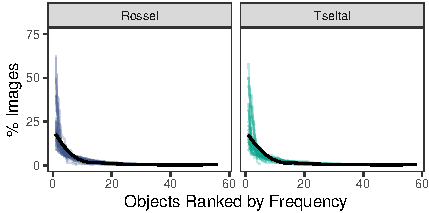
\includegraphics{figs/zipfian-objects-fig-1} 

}

\caption[Zipfian distribution of objects handled by each child across sites]{Zipfian distribution of objects handled by each child across sites. For each child, the top object was defined as the object appearing in the greatest number of images; thus, the identity of the top object does not match across all children.}\label{fig:zipfian-objects-fig}
\end{figure}
\end{CodeChunk}

Comparing across sites, 33.62\% of objects were handled by both Rossel
and Tseltal children, and several shared objects were among the most
frequently handled in both sites. In fact, among the top 25 most common
objects, 10 were shared across sites (Figure 3). Of note, the study
camera was the object that was handled by the most children in both
sites (Rossel: 69.2\%, Tseltal: 91.4\% of children, see Bergelson,
Amatuni, Dailey, Koorathota, \& Tor, 2019, for a similar effect) but
accounted for a relatively small percentage of each child's object
handling time, on average (\emph{M}\textsubscript{\emph{Rossel}} =
3.8\%, \emph{M}\textsubscript{\emph{Tseltal}} = 6.5\% of images). The
camera and other study-related objects (i.e., vest and privacy cover for
the camera), were retained in our analyses; however, inclusion of these
items did not qualitatively change any of the reported results.

\begin{CodeChunk}
\begin{figure*}[!ht]

{\centering 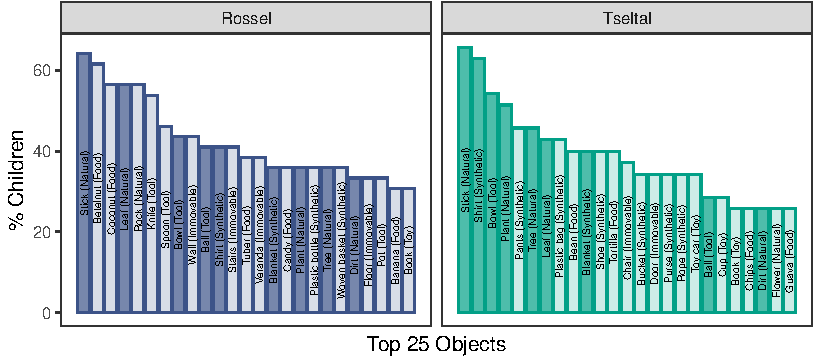
\includegraphics{figs/top-objects-fig-1} 

}

\caption[Non-study-related objects handled at least once by the most children in each site]{Non-study-related objects handled at least once by the most children in each site. Filled bars represent objects that were among the top 25 for both sites.}\label{fig:top-objects-fig}
\end{figure*}
\end{CodeChunk}

\hypertarget{effects-of-object-category}{%
\subsection{Effects of object
category}\label{effects-of-object-category}}

We quantify the distribution of object categories at two timescales:
across the whole waking day (i.e., overall \% handling for different
object categories across all images) and across individual hours (i.e.,
number of unique objects from different object categories per hour).

The overall frequency of object categories was similarly divided across
sites (Figure 4A). Children primarily handled food items
(\emph{M}\textsubscript{\emph{Rossel}} = 25.68\%,
\emph{M}\textsubscript{\emph{Tseltal}} = 30.93\% of handling) and
miscellaneous synthetic objects (\emph{M}\textsubscript{\emph{Rossel}} =
24.41\%, \emph{M}\textsubscript{\emph{Tseltal}} = 31.11\% of handling).
For 51 of 75 children, their top category was either food or synthetic
objects. Two-tailed Wilcoxon tests revealed no significant
category-level differences between sites after correcting for multiple
comparisons (all adjusted \emph{p}s \textgreater0.05). The only
categories trending toward difference were as follows: more handling of
synthetic objects by Tseltal children
(\emph{M}\textsubscript{\emph{Rossel}} = 24.41\%,
\emph{M}\textsubscript{\emph{Tseltal}} = 31.11\%), and more handling of
mealtime tools (\emph{M}\textsubscript{\emph{Rossel}} = 10.36\%,
\emph{M}\textsubscript{\emph{Tseltal}} = 8.1\%) and immovable objects
(\emph{M}\textsubscript{\emph{Rossel}} = 7.53\%,
\emph{M}\textsubscript{\emph{Tseltal}} = 2.52\%) by Rossel children.

\begin{CodeChunk}
\begin{figure}[!h]

{\centering 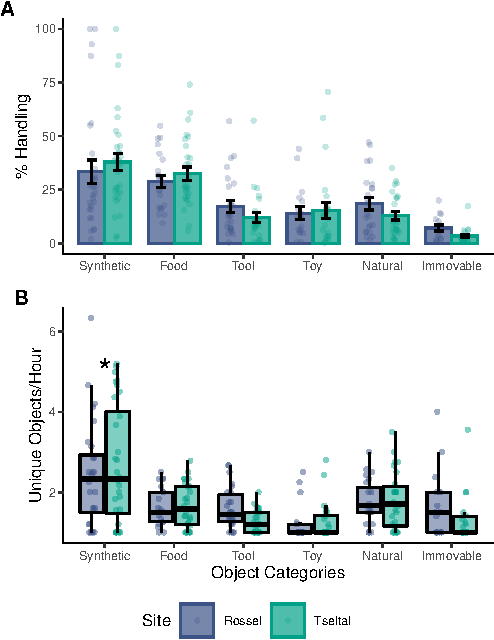
\includegraphics{figs/overall-stats-fig-1} 

}

\caption[(A) Overall frequency of handling by object category]{(A) Overall frequency of handling by object category. Points reflect percentages for individual children. (B) Count of unique objects handled per hour by object category. Points reflect means for individual children across all hours of recording. Asterisks indicate significant differences between sites after correcting for multiple comparisons.}\label{fig:overall-stats-fig}
\end{figure}
\end{CodeChunk}

During any given hour, children handled 4.84 objects from 2.75 different
categories, on average (median = 3.00 objects, \emph{SD} = 4.89, range =
0--27). To test for differences across sites and categories, we ran
individual linear mixed-effects models for each of the eight object
categories, with category membership dummy coded (i.e., objects
belonging to the target category for a given model = 1, objects
belonging to other categories = 0). Each regression model included fixed
effects of site, category, number of images, and a site-by-category
interaction as well as random intercepts for individual children. After
correcting for multiple comparisons, we found a significant main effect
of the synthetic object category (\(\beta\) = 0.34, \emph{SE} = 0.09,
\emph{t} = 3.86, \emph{p} = 0.003) and a marginal site-by-synthetic
interaction (\(\beta\) = 0.37, \emph{SE} = 0.12, \emph{t} = 2.99,
\emph{p} = 0.054) such that children handled more unique synthetic
objects per hour than objects from other categories, and this effect was
stronger for Tseltal children than for Rossel children. Additionally, we
found negative main effects for the toy (\(\beta\) = -0.41, \emph{SE} =
0.13, \emph{t} = -3.08, \emph{p} = 0.042) and work tool (\(\beta\) =
-0.63, \emph{SE} = 0.17, \emph{t} = -3.71, \emph{p} = 0.005) categories,
indicating that children handled fewer unique objects from these
categories per hour relative to other categories. Finally, a significant
main effect of the immovable object category (\(\beta\) = 0.47,
\emph{SE} = 0.11, \emph{t} = 4.24, \emph{p} \textless{} 0.001) and a
significant site-by-immovable interaction (\(\beta\) = -0.84, \emph{SE}
= 0.17, \emph{t} = -4.85, \emph{p} \textless{} 0.001) revealed that
children handled more unique immovable objects per hour than objects
from other categories, and this effect was stronger for Rossel children
than for Tseltal children (Figure 4B).

\hypertarget{effects-of-age}{%
\subsection{Effects of age}\label{effects-of-age}}

Prior work with the same data set indicated a significant increase in
object handling across the first four years (Casillas \& Elliott, 2021).
By adding information about \emph{what} objects children are handling,
we can now explore finer-grained characteristics of age-related change
in object handling. We investigate age-related changes in (a) the
distribution of object categories, (b) the number of unique objects and
categories handled per hour, and (c) transitions between objects and
categories per hour.

\emph{Do children handle different objects with age?} We fit individual
linear regressions predicting the proportion of handling time for each
category as a function of age (in months), site, and their interaction.
We included number of images as an additional fixed effect to account
for the wide range in total available images for each child (range =
1--584), leading to some proportions close to 0 or 1 that are based on
only a handful of images\footnote{As expected, number of handling images
  was correlated with age (\emph{r} = 0.49 {[}0.30, 0.65{]}, \emph{p}
  \textless{} 0.001), which we attribute to changes in motor development
  and permitted object access over the first four years (Casillas \&
  Elliott, 2021)---the correlation is an artifactual outcome of
  development. Including both as fixed effects in a regression poses no
  technical issue in estimating \(R^{2}\), but does limit the total
  variance attributed independently to either variable (Wurm \&
  Fisicaro, 2014). Thus, for models of non-proportional measures, we
  rely solely on age to capture this variance.}. This analysis revealed
no significant age-related changes in the frequency of handling of
different object categories and no significant site-by-age interaction
effects (all adjusted \emph{p}s \textgreater{} 0.05). Thus, the the
broad composition of handled objects remained largely stable over age
(Figure 5).

\begin{CodeChunk}
\begin{figure}[!ht]

{\centering 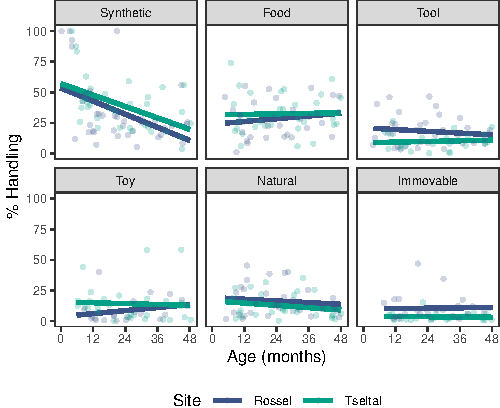
\includegraphics{figs/age-effects-bycategory-fig-1} 

}

\caption[Frequency of handling by object category across age]{Frequency of handling by object category across age. Individual points show raw percentages per hour for each child, and lines reflect model-predicted percentages.}\label{fig:age-effects-bycategory-fig}
\end{figure}
\end{CodeChunk}

\emph{Does object handling diversify with age?} In addition to the
overall age-related increase in handling found by Casillas and Elliott
(2021), we see that, with increasing age, children handled more unique
objects per hour (\(\beta\) = 0.11, \emph{SE} = 0.03, \emph{t} = 3.14,
\emph{p} = 0.002; Figure 6A) and more objects from different categories
per hour (\(\beta\) = 0.05, \emph{SE} = 0.01, \emph{t} = 4.02, \emph{p}
= 0). These effects were consistent across sites; we found no main
effects of site or interactions between site and age (all \emph{p}s
\textgreater{} 0.05).

\emph{Does object handling become more complex with age?} Analysis of
children's relative rate of transition between objects per hour (i.e.,
the number of transitions from one object to another divided by the
number of available objects for that hour) did not reveal an overall
age-related increase (\(\beta\) = 0.01, \emph{SE} = 0, \emph{t} = 1.59,
\emph{p} = 0.117). However, there was a significant main effect of site
(\(\beta\) = -0.45, \emph{SE} = 0.14, \emph{t} = -3.21, \emph{p} =
0.002) as well as a site-by-age interaction (\(\beta\) = 0.01, \emph{SE}
= 0.01, \emph{t} = 2.55, \emph{p} = 0.013), indicating that Tseltal
children made fewer transitions between objects per hour than Rossel
children but showed a steeper increase across age (Figure 6B). At the
category level, we found that, children made marginally more transitions
between object categories per hour with age (\(\beta\) = 0.02, \emph{SE}
= 0.01, \emph{t} = 1.94, \emph{p} = 0.056), with no detectable
differences across sites.

\begin{CodeChunk}
\begin{figure}[!ht]

{\centering 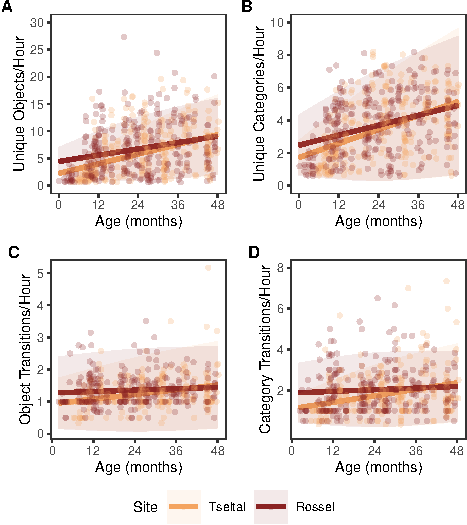
\includegraphics{figs/age-effects-fig-1} 

}

\caption[(A) Unique objects handled per hour as a function of age]{(A) Unique objects handled per hour as a function of age. (B) Relative number of transitions between objects per hour as a function of age. Points reflect raw hourly counts for each child, and lines reflect model predictions with shaded standard error regions.}\label{fig:age-effects-fig}
\end{figure}
\end{CodeChunk}

\hypertarget{discussion}{%
\section{Discussion}\label{discussion}}

We discuss this rich set of findings with respect to (a) object handling
as a viewpoint into children's worlds in general and (b) the
implications of our findings for word learning specifically.

\hypertarget{objects-as-insight-into-childrens-worlds}{%
\subsection{Objects as insight into children's
worlds}\label{objects-as-insight-into-childrens-worlds}}

The total time children spend handling objects of different types (e.g.,
natural, immovable, synthetic, etc.) is stable across age and sites
(consistent with Long, Kachergis, Bhatt, \& Frank, 2021 for visually
present categories). Specifically, food and synthetic objects dominate
over others across age. We suggest that this measure, total time spent
within categories, may reflect stable properties of the environment and
routines children engage in across age and across diverse contexts. If
we continued to sample in other communities we would expect to find more
differences (e.g., the time spent with toys in US middle-class samples),
but these two rural subsistence communities show overall similar
profiles despite differences in market integration, the organization of
daily life, infant carrying, and other aspects of these cultural milieux
(Brown \& Casillas, 2021; Casillas, Brown, \& Levinson, 2020, 2021;
Casillas \& Elliott, 2021).

The individual objects children handle reveals strong age-related change
as well as some site-related differences. Children's object handling
diversifies within and across categories as they get older, which means
more unique objects held, objects from more categories, and,
concomitantly, more frequent transitions between objects. Note that this
effect may be stronger for the Tseltal children who are more restricted
in their movements in early infancy because they are carried in a sling
(Casillas \& Elliott, 2021). Compared to other categories, we see
children handling a greater diversity of synthetic objects (stronger for
Tseltal) and immovable objects (stronger for Rossel) per hour compared
to other categories, reflecting the greater market integration (and
hence availability of diverse synthetic objects) of the Tseltal
community and the long daily periods of socializing around family
verandas in the Rossel community.

We suggest that the individual objects children handle gives us insight
into maturity via children's increased engagement and access to the
wider range of objects associated with everyday activities (e.g., not
just holding finger food at meals, but also using a spoon, passing a
bowl, etc.) and to the greater diversity of objects associated with
economically or culturally variable facets of everyday life (e.g., a
variety of toys available for purchase nearby, climbable surfaces where
daily socializing takes place)

\hypertarget{implications-for-word-learning}{%
\subsection{Implications for word
learning}\label{implications-for-word-learning}}

These data indicate that children are exposed to a stable and wide
variety of object categories in the first four years of life, with
increasing access to a diversity of objects within categories as they
get older. Similarity in the distribution of object categories across
sites suggests some basis for expecting similarity in early object label
knowledge by children in these two sites. Individual objects also show a
Zipfian distribution in how they are handled, with some handled
frequently and most handled infrequently; may be good for word learning
(see also Carvalho, Chen, \& Yu, 2019; Clerkin, Hart, Rehg, Yu, \&
Smith, 2017; Long, Kachergis, Bhatt, \& Frank, 2021; Montag, Jones, \&
Smith, 2018) and, in tandem with these other effects across age and
cultural context, may indicate which words for objects children are
likely to learn first and how their semantic networks grow within and
across categories.

The overarching story is one where children's early object-centric
interactions are anchored on a few unique items across the different
categories relevant to daily life, similar to other accounts of how kids
get into segmentation, etc. What we need to know, however, is how often
these objects are labeled for or by children as they interact with them,
and how the labeling behavior itself fluctuates across age, activity,
and cultural context.

\hypertarget{references}{%
\section{References}\label{references}}

\setlength{\parindent}{-0.1in} 
\setlength{\leftskip}{0.125in}

\noindent

\hypertarget{refs}{}
\begin{CSLReferences}{1}{0}
\leavevmode\hypertarget{ref-adolph2010motor}{}%
Adolph, K. E., Karasik, L. B., \& Tamis-LeMonda, C. S. (2010). Motor
skill. In M. H. Bornstein (Ed.), \emph{Handbook of cultural
developmental science} (pp. 61--88). Psychology Press: New York, NY.

\leavevmode\hypertarget{ref-arnold2012life}{}%
Arnold, J. E., Graesch, A. P., Ochs, E., \& Ragazzini, E. (2012).
\emph{Life at home in the twenty-first century: 32 families open their
doors}. ISD LLC.

\leavevmode\hypertarget{ref-bergelson2019day}{}%
Bergelson, E., Amatuni, A., Dailey, S., Koorathota, S., \& Tor, S.
(2019). Day by day, hour by hour: Naturalistic language input to
infants. \emph{Developmental Science}, \emph{22}(1), e12715.

\leavevmode\hypertarget{ref-bergelson2017nature}{}%
Bergelson, E., \& Aslin, R. N. (2017). Nature and origins of the lexicon
in 6-mo-olds. \emph{Proceedings of the National Academy of Sciences},
\emph{114}(49), 12916--12921.

\leavevmode\hypertarget{ref-brownIPchildrearing}{}%
Brown, P., \& Casillas, M. (2021). \emph{Childrearing through social
interaction on {Rossel Island, PNG}}. (A. J. Fentiman \& M. Goody,
Eds.). New York, NY: Berghahn.

\leavevmode\hypertarget{ref-carvalho2019rethinking}{}%
Carvalho, P., Chen, C., \& Yu, C. (2019). \emph{Rethinking the input:
Skewed distributions of exemplars result in broad generalization in
category learning}.

\leavevmode\hypertarget{ref-casey2022imco}{}%
Casey, K., Fisher, W., Tice, S. C., \& Casillas, M. (2022). ImCo: A
python tkinter application for coding lots of images (Version 2.0).
Retrieved from \url{https://github.com/kennedycasey/ImCo2}

\leavevmode\hypertarget{ref-casillas2020early}{}%
Casillas, M., Brown, P., \& Levinson, S. C. (2020). Early language
experience in a {Tseltal Mayan} village. \emph{Child Development},
\emph{91}(5), 1819--1835.

\leavevmode\hypertarget{ref-casillas2021early}{}%
Casillas, M., Brown, P., \& Levinson, S. C. (2021). Early language
experience in a papuan community. \emph{Journal of Child Language},
\emph{48}(4), 792--814.

\leavevmode\hypertarget{ref-casillasURdaylong}{}%
Casillas, M., \& Elliott, M. (2021). Cross-cultural differences in
children's object handling at home. PsyArXiv.
http://doi.org/\href{https://doi.org/10.31234/osf.io/43db8}{10.31234/osf.io/43db8}

\leavevmode\hypertarget{ref-clerkin2017real}{}%
Clerkin, E. M., Hart, E., Rehg, J. M., Yu, C., \& Smith, L. B. (2017).
Real-world visual statistics and infants' first-learned object names.
\emph{Philosophical Transactions of the Royal Society B: Biological
Sciences}, \emph{372}(1711), 20160055.

\leavevmode\hypertarget{ref-fausey2016faces}{}%
Fausey, C. M., Jayaraman, S., \& Smith, L. B. (2016). From faces to
hands: Changing visual input in the first two years. \emph{Cognition},
\emph{152}, 101--107.

\leavevmode\hypertarget{ref-gaskins2000childrens}{}%
Gaskins, S. (2000). Children's daily activities in a {M}ayan village: A
culturally grounded description. \emph{Cross-Cultural Research},
\emph{34}(4), 375--389.

\leavevmode\hypertarget{ref-herzberg2021exuberant}{}%
Herzberg, O., Fletcher, K. K., Schatz, J. L., \& Tamis-LeMonda, C. S.
(2021). Infant exuberant object play at home: Immense amounts of
time-distributed, variable practice. \emph{Child Development},
\emph{XX}, 1--15.

\leavevmode\hypertarget{ref-jayaraman2017faces}{}%
Jayaraman, S., Fausey, C. M., \& Smith, L. B. (2017). Why are faces
denser in the visual experiences of younger than older infants?
\emph{Developmental Psychology}, \emph{53}(1), 38.

\leavevmode\hypertarget{ref-karasik2018not}{}%
Karasik, L. B., Schneider, J., Kuchirko, Y. A., \& Tamis-LeMonda, C. S.
(2018). Not so {WEIRD} object play in {T}ajikistan. Presentation to the
International Conference on Infant Studies, Philadelphia, PA.
http://doi.org/\href{https://doi.org/10.31234/osf.io/43db8}{10.31234/osf.io/43db8}

\leavevmode\hypertarget{ref-kretch2014crawling}{}%
Kretch, K. S., Franchak, J. M., \& Adolph, K. E. (2014). Crawling and
walking infants see the world differently. \emph{Child Development},
\emph{85}(4), 1503--1518.

\leavevmode\hypertarget{ref-laing2020babble}{}%
Laing, C., \& Bergelson, E. (2020). From babble to words: Infants' early
productions match words and objects in their environment.
\emph{Cognitive Psychology}, \emph{122}, 101308.

\leavevmode\hypertarget{ref-long2020detecting}{}%
Long, B., Kachergis, G., Agrawal, K., \& Frank, M. C. (2020).
\emph{Detecting social information in a dense database of infants'
natural visual experience}.

\leavevmode\hypertarget{ref-long2021characterizing}{}%
Long, B., Kachergis, G., Bhatt, N., \& Frank, M. C. (2021).
\emph{Characterizing the object categories two children see and interact
within a dense dataset of naturalistic visual experience}.

\leavevmode\hypertarget{ref-montag2018quantity}{}%
Montag, J. L., Jones, M. N., \& Smith, L. B. (2018). Quantity and
diversity: Simulating early word learning environments. \emph{Cognitive
Science}, \emph{42}, 375--412.

\leavevmode\hypertarget{ref-sanchez2018detecting}{}%
Sanchez, A., Long, B., Kraus, A. M., \& Frank, M. C. (2018). Postural
developments modulate children's visual access to social information. In
\emph{Proceedings of the 40th annual conference of the cognitive science
society} (pp. 2412--2417).

\leavevmode\hypertarget{ref-slone2019self}{}%
Slone, L. K., Smith, L. B., \& Yu, C. (2019). Self-generated variability
in object images predicts vocabulary growth. \emph{Developmental
Science}, \emph{22}(6), e12816.

\leavevmode\hypertarget{ref-super1976environmental}{}%
Super, C. M. (1976). Environmental effects on motor development: The
case of {`{A}frican infant precocity.'} \emph{Developmental Medicine \&
Child Neurology}, \emph{18}(5), 561--567.

\leavevmode\hypertarget{ref-wurm2014residualizing}{}%
Wurm, L. H., \& Fisicaro, S. A. (2014). What residualizing predictors in
regression analyses does (and what it does not do). \emph{Journal of
Memory and Language}, \emph{72}, 37--48.

\leavevmode\hypertarget{ref-yu2013joint}{}%
Yu, C., \& Smith, L. B. (2013). Joint attention without gaze following:
Human infants and their parents coordinate visual attention to objects
through eye-hand coordination. \emph{PloS One}, \emph{8}(11), e79659.

\leavevmode\hypertarget{ref-yurovsky2013statistical}{}%
Yurovsky, D., Smith, L. B., \& Yu, C. (2013). Statistical word learning
at scale: The baby's view is better. \emph{Developmental Science},
\emph{16}(6), 959--966.

\end{CSLReferences}

\bibliographystyle{apacite}


\end{document}
